% !TEX root = ../dissertacao.tex
% \acresetall{}
\chapter{Explorando a localidade espacial dos dados}
\label{cap:tecnica_proposta}

Este capítulo apresenta a proposta de organização dos dados para melhorar o desempenho de algoritmos.
Inicialmente, são discutidas as limitações do modelo \ac{ood} e o de como o modelo \ac{dod} pode sanar as mesmas.
Então, na Seção~\ref{sec:entity_component_system} é apresentado um padrão de projeto que segue o modelo \ac{dod} e otimiza a localidade espacial dos dados, otimizando assim os acessos à memória realizados pelas tarefas.

% A arquitetura de memória de computadores modernos é tipicamente hierárquica como mostrado na Figura~\ref{fig:memoryHierarchy}. Observe que os níveis mais baixos na hierarquia (por exemplo, disco rígido e memória principal) têm maior capacidade porém, possuem maior latência. Por outro lado, os níveis mais altos (por exemplo, memória cache e registradores da CPU) são rápidos, mas possuem capacidade limitada. Quando um determinado programa precisa um dado, e o mesmo não se encontra nos registradores da CPU, será realizada uma busca por este dado nos níveis mais altos da hierarquia da  cache. Quando os dados não são encontrados em algum dos níveis de cache, dizemos que ocorreu um \textbf{\textit{cache miss}}. Quando um \textit{cache miss} ocorre, os dados são acessados no nível inferior da hierarquia. No pior caso, este dado será recuperado do disco rígido e levado por todos os níveis da hierarquia. Quando o dado buscado é recuperado para a cache de mais alto nível e posteriormente armazenado num registrador da CPU, o programa que estava acessando os dados volta a executar. Caso esses dados forem necessários novamente, e o bloco da cache não tenha sido substituído, eles estarão disponível na cache e sua busca nos níveis da cache resultará em \textbf{\textit{cache hit}}~\cite{patterson2013computer}.

% \begin{figure}[ht]
%     \centering
%     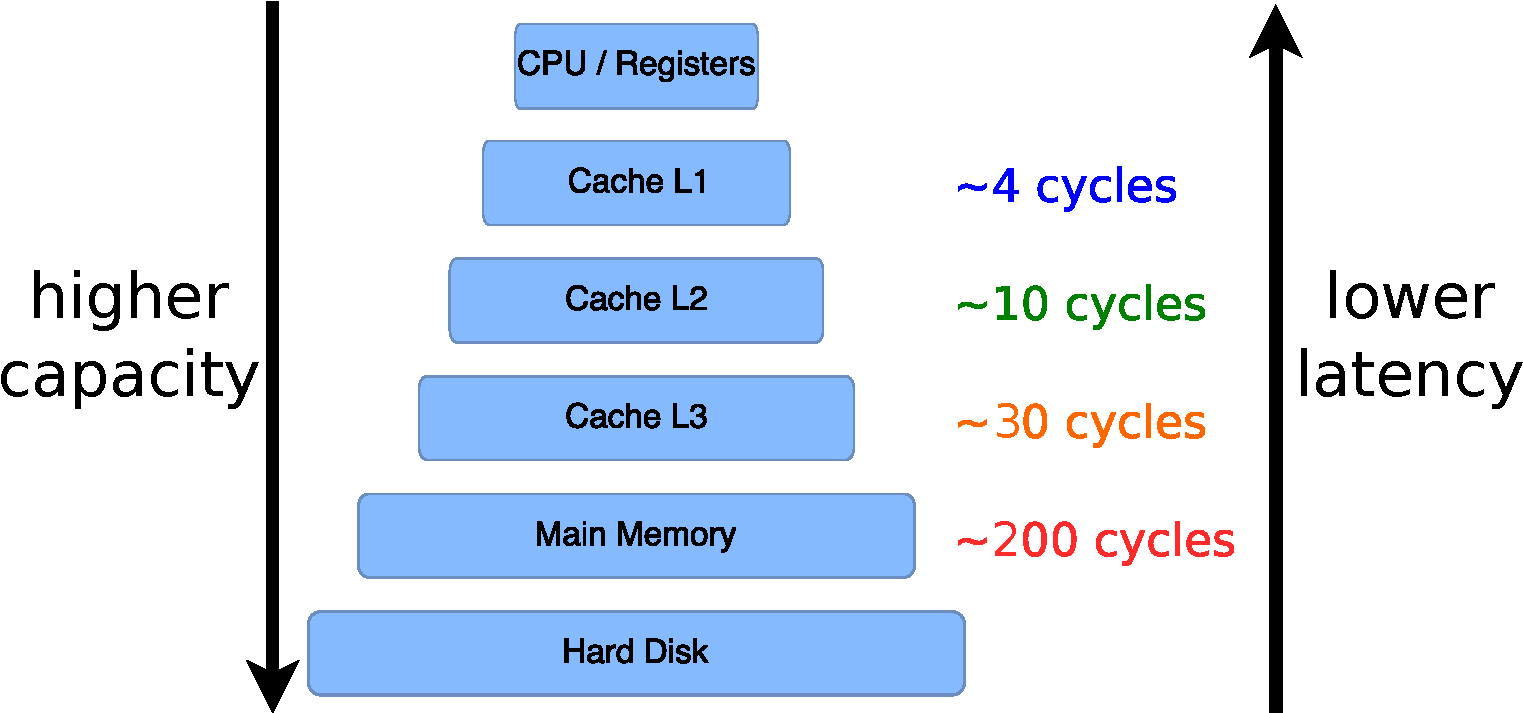
\includegraphics[width=0.7\linewidth]{img/tecnica/memoryHierarchy}
%     % \caption{Hierarchy of memory present in modern computers. The hierarchy is compose by hard disk, main memory, three levels of cache and CPU registers. Adapted from~\cite{patterson2013computer}.}
%     % \caption[Hierarquia de memória]{Hierarquia de memória presente em computadores modernos. A hierarquia é composta por disco rígido, memória principal, três níveis de cache e registradores. Adaptada de~\cite{patterson2013computer}.}
%     \caption[Hierarquia de memória]{Hierarquia de memória presente em computadores modernos. Adaptada de~\cite{patterson2013computer}.}
%     \label{fig:memoryHierarchy}
% \end{figure}


% A localidade espacial (\textit{spatial locality}) é uma propriedade importante dos sistemas hierárquicos de memória. Esta propriedade afirma que a probabilidade de acessar uma posição da memória é maior se uma posição próxima já foi referenciada~\cite{patterson2013computer}. O sistema de cache explora esta propriedade armazenando os dados em blocos (\textit{cache blocks}). Sempre que algum dado é acessado a partir da memória principal, ele é recuperado para a cache juntamente com outros dados que estavam armazenados próximos a ele. Desta forma, se os dados próximos forem acessados posteriormente, resultarão em \textit{cache hits}.

Como revisado na Seção~\ref{sec:conceitosFundamentaisArquitetura}, a arquitetura de computadores modernos possui um hierarquia de memória.
Esta hierarquia de memória possui algumas propriedades, sendo uma delas a localidade espacial.
É possível explorar esta propriedade mudando a forma como os dados são organizados em um determinado \textit{software}, até mesmo quando não se possui informação da arquitetura na qual este \textit{software} irá executar.
Isto é possível, uma vez que, ao armazenar dados de uma mesma categoria de forma contígua estamos aumentando a probabilidade de um acesso gerar um \textit{cache hit}.

Por exemplo, no contexto da síntese física, um algoritmo de Clusterização de Registradores executa operações em todas as posições dos registradores de um circuito.
Ao armazenar todas as posições destes registradores em um único vetor contíguo, este algoritmo irá incorrer em um número inferior de \textit{cache misses} para recuperar todos os dados.
Como consequência, o tempo de acesso aos dados é reduzido e o desempenho do \textit{software} é melhorado. Esta organização de dados nem sempre é eficientemente feita pelo modelo de programação~\ac{ood}.
Neste modelo de programação, os dados são armazenados agrupando-se todas as informações de um mesmo objeto num único registro.
Observe que com esta abordagem, quando os objetos são recuperados para a \textit{cache}, alguns dados inúteis (atributos do objeto) são carregados junto.
Portanto, parte do espaço da memória \textit{cache} é desperdiçado com dados que não serão utilizados pelo algoritmo.

% Uma alternativa para o modelo de \ac{ood} é o modelo de programação \ac{dod}. Este modelo tem como enfoque a forma como os dados são organizados na memória.
% % A Figura~\ref{fig:entityPropertyDOD} mostra um exemplo sobre como modelar os dados usando este modelo de programação.
% Enquanto no modelo \ac{ood} utiliza objetos complexos e seus atributos para representar os objetos do mundo real, o modelo \ac{dod} representa os dados do mundo real como entidades e suas propriedades (atributos).
% Cada entidade é simplesmente um índice. Este índice é utilizado para acessar suas propriedades.
% Assim, cada propriedade pode ser armazenada num único vetor contíguo na memória.
% % Por exemplo, na Figura~\ref{fig:entityPropertyDOD}, o vetor de entidades armazenam todos os índices das entidade, enquanto os outros vetores armazenam suas propriedades, as quais podem ser acessadas usando os índices do vetor de entidades.
% Ao organizar os dados dessa forma, quando um algoritmo precisa apenas de uma propriedade (por exemplo a posição dos registradores) ele pode recuperar somente o vetor que contem estes dados.
% Desta forma, não são recuperados dados desnecessários o que acarreta numa maior localidade espacial da cache.

% \begin{figure}[ht]
%     \centering
%     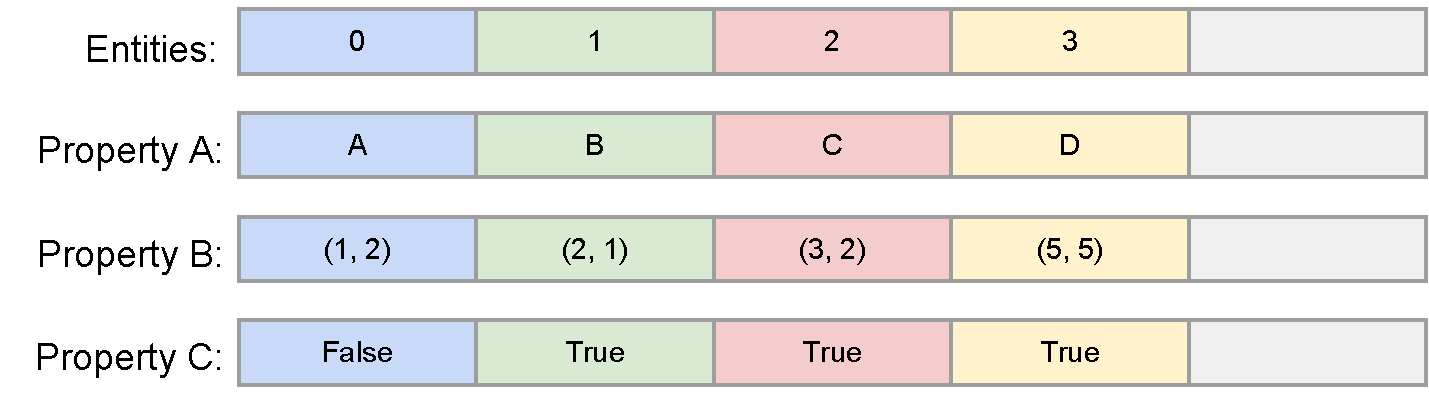
\includegraphics[width=0.7\linewidth]{img/tecnica/entityPropertyDOD}
%     % \caption{Modeling entities and their properties with \ac{dod} approach.}
%     \caption[Exemplo de entidades DOD]{Exemplo de entidades e suas propriedades seguindo o modelo de programação DOD.}
%     \label{fig:entityPropertyDOD}
% \end{figure}

Com o objetivo de explanar como a organização dos dados pode impactar na utilização da memória \textit{cache}, a Figura~\ref{fig:cache_register_clustering} apresenta um comparativo entre duas organizações de dados para a mesma funcionalidade. 
Nesta figura são apresentados trechos de códigos (lado esquerdo) para cada organização e um bloco da \textit{cache} após a execução (lado direito).
A Figura~\ref{fig:cache_register_clustering}~(a) representa a modelagem dos dados seguindo a abordagem \ac{aos}, que é utilizada na orientação a objetos (OOD).
A Figura~\ref{fig:cache_register_clustering}~(b) representa a abordagem \ac{soa}, utilizada no modelo orientado a dados (DOD).
Admita que, para ambos os casos, a \textit{cache} apresentada possui blocos com tamanho de $128$ $bytes$, cada número inteiro ocupa $4$ $bytes$ e, por motivos de simplicidade, cada palavra (\textit{string}) ocupa $8$ $bytes$. 


\begin{figure}[h!t]
    \subfigure[Array of Structures (AoS)]{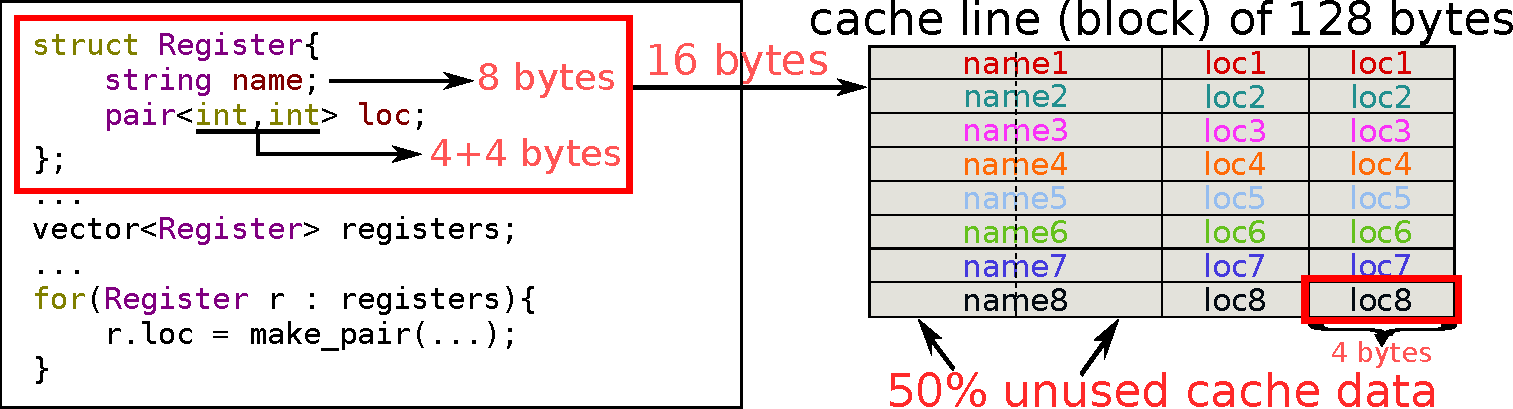
\includegraphics[width=\linewidth]{img/tecnica/cacheUtilizationRegisterClusterclassOOD}}
    % to break figure
    \subfigure[Structure of Arrays (SoA)]{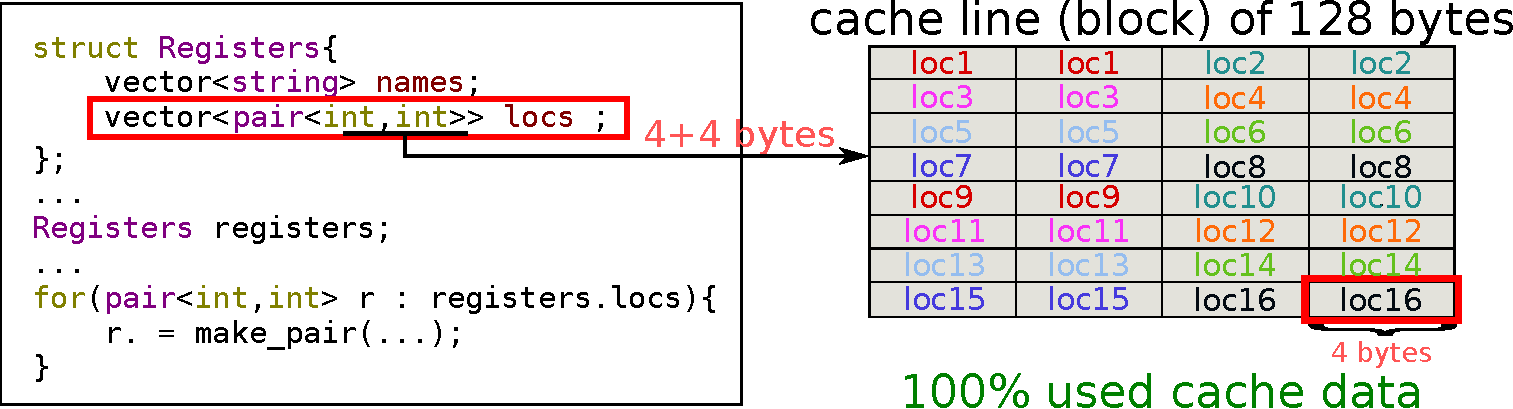
\includegraphics[width=\linewidth]{img/tecnica/cacheUtilizationRegisterClusterclassDOD}}
    \caption[Comparação da utilização da \textit{cache}]{Comparação da utilização da \textit{cache} para diferentes modelos de organização dos dados.}
    \label{fig:cache_register_clustering}
\end{figure}

Pode-se notar que no modelo \ac{ood}, quando ocorre um \textit{cache miss}, todo o objeto precisa ser recuperado para a \textit{cache}. Ao recuperar todas as informações do objeto, desperdiça-se espaço com atributos/informações que não serão utilizados na solução do problema. No exemplo da Figura~\ref{fig:cache_register_clustering}~(a) são carregados para a \textit{cache} os nomes e as posições dos registradores (Struct Register). Porém, considerando que se desejasse alterar somente as posições dos registradores, $50\%$ dos dados recuperados por um \textit{cache miss} seriam desperdiçados.



Utilizando-se o modelo \ac{dod}, Figura~\ref{fig:cache_register_clustering}~(b), quando um \textit{cache miss} ocorre, somente o vetor das propriedades necessárias é recuperado para a \textit{cache}. Este fato implica que atributos desnecessários para esta execução não serão recuperados. Assim, a memória \textit{cache} será preenchida somente com dados úteis.
Seguindo esta abordagem, o número de \textit{cache misses} será menor e consequentemente, o tempo de acesso aos dados da memória principal será reduzido. Estes fatores poderão contribuir para reduzir o tempo total despendido por uma aplicação para executar determinado algoritmo.



% Para exemplificar a diferença entre os modelos \ac{ood} e \ac{dod} na modelagem dos dados, a Figura~\ref{fig:modelo_register_clustering} apresenta uma possível solução para o problema de clusterização de registradores seguindo estes dois modelos.
O uso de DOD também impacta em diferenças na modelagem dos dados. Por exemplo, a Figura~\ref{fig:modelo_register_clustering} apresenta uma possível solução para o problema de clusterização de registradores seguindo estes dois modelos.
Na Figura~\ref{fig:modelo_register_clustering}~(a) é apresentado o diagrama de classes do problema com orientação a objetos. Nesta modelagem são necessárias duas classes: uma para representar os registradores (\textit{Register}) e outra para representar os clusters (\textit{Cluster}). Ambas as classes possuem dois atributos. A classe \textit{Cluster} possui a posição de seu centro e os registradores que pertencem ao cluster. A classe \textit{Register}, por sua vez, possui o nome e a posição do registrador.

\begin{figure}[h!t]
    \centering
    \subfigure[OOD]{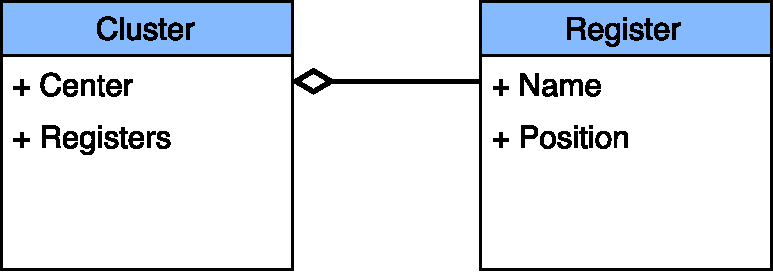
\includegraphics[width=0.5\linewidth]{img/tecnica/registerClusterclassOOD}}
    % to break figure
    \subfigure[DOD]{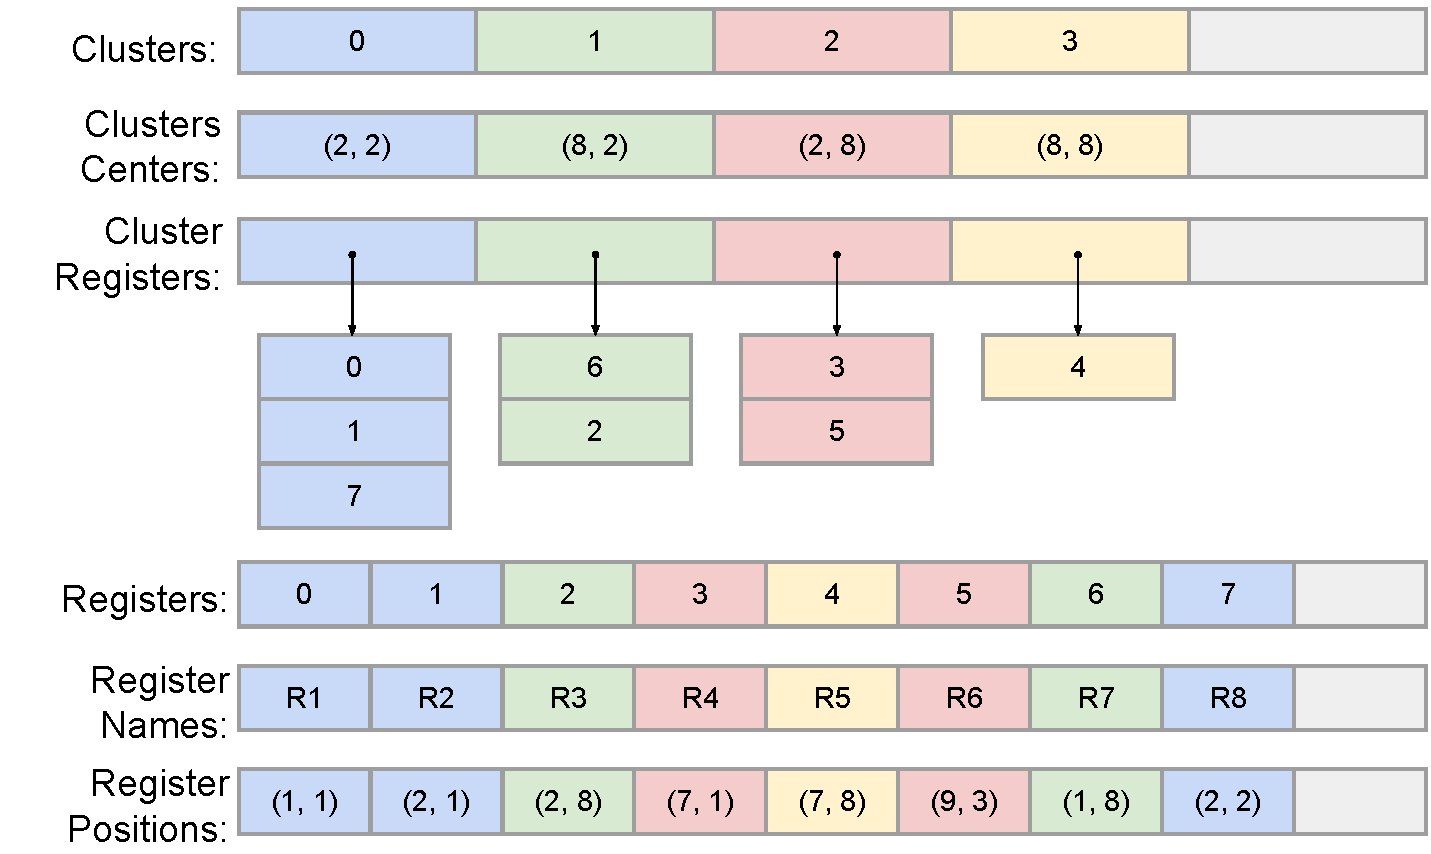
\includegraphics[width=0.8\linewidth]{img/tecnica/registerClusterclassDOD}}
    \caption{Modelagem dos dados para clusterização de registradores.}
    \label{fig:modelo_register_clustering}
\end{figure}


A Figura~\ref{fig:modelo_register_clustering}~(b) representa os mesmos dados da Figura~\ref{fig:modelo_register_clustering}~(a) porém, seguindo o modelo de programação \ac{dod}.
% Nesta figura cada cor representa uma instância que seria criada no modelo orientado a objetos. Os vetores \textit{Clusters} e \textit{Registers} armazenam contiguamente os indices dos objetos.
Nesta figura cada linha representa um vetor.
Cada atributo criado no modelo \ac{ood} é aqui representado por uma propriedade, cujo armazenamento é realizado de forma contígua em um único vetor.
Os vetores ``\textit{Clusters}'' e ``\textit{Registers}'' armazenam as entidades, sendo os demais vetores as propriedades destas entidades.
Estas propriedades serão agora recuperadas a partir do índice de uma entidade.
Por exemplo, a posição de um registrador $i$ é recuperada acessando o vetor ``\textit{Register Positions}'' na posição $i$.

Embora o modelo \ac{dod} possa reduzir o número de \textit{cache misses}, seu conceito não é trivial de adotar.
Para usar eficientemente este modelo de programação, é necessário gerenciar os vetores de propriedades para garantir que os mesmos permaneçam contíguos à medida que novos dados são adicionados e/ou removidos. Um padrão de projeto chamado Sistema de Componente e Entidade (\textit{Entity-Component System}) pode ser adotado para lidar com esse problema~\cite{nystrom2014game}. Este padrão de projeto é descrito na seção a seguir.

\section{\textit{Entity-Component System}}
\label{sec:entity_component_system}

Esta seção traz os conceitos envolvidos no padrão de projetos \textit{Entity-Component System}.
Primeiramente, serão explicados o que são Entidades e Componentes e qual a sua relação com o padrão de projeto \ac{ood}.
A seguir, aborda-se o gerenciamento das entidades para que operações elementares ocorram em tempo computacional constante.

\subsection{Entidades e Componentes}

O padrão de projeto \textit{Entity-Component System} consiste em decompor um problema em um conjunto de entidades e seus componentes~\cite{nystrom2014game}. As entidades são análogas aos objetos no modelo \ac{ood}, enquanto os componentes correspondem às suas propriedades (ou atributos). Neste trabalho, os componentes serão referenciados por propriedades. Díspar aos objetos, as entidades não são estruturas complexas, elas são apenas identificadores únicos (IDs). Cada propriedade, por sua vez, é representada usando um vetor de dados. O índice (ID) da entidade é utilizado para acessar suas propriedades nesses vetores. Por exemplo, a Figura~\ref{fig:entity_example} ilustra uma entidade com cinco propriedades, onde cada propriedade corresponde a um vetor e o ID da entidade é utilizado para acessar todos os vetores. Da mesma forma que as propriedades, cada uma dessas entidades é armazenada em um vetor contíguo.

\begin{figure}[ht]
    \centering
    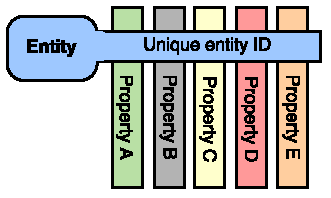
\includegraphics[width=0.5\linewidth]{img/tecnica/entity}
    % \caption{Example of entity with five properties. The entity id is used to access the information of all properties.}
    \caption[Exemplo de uma entidade]{Exemplo de uma entidade com cinco propriedades. O índice (ID) da entidade é utilizado para acessar as informações de todas as propriedades.}
    \label{fig:entity_example}
\end{figure}

\subsection{Sistema de Entidades}

O sistema de entidades é necessário para gerenciar o acesso às entidades e suas propriedades. Este sistema também é responsável por criar e destruir entidades, bem como gerenciar os vetores das propriedades ao alterar o número de entidades. Por exemplo, se uma entidade for criada ou destruída, o sistema da entidade deve assegurar, de forma eficiente, que todos os vetores permanecem contíguos na memória.

Além de gerenciar a criação e destruição de entidades, o sistema de entidade deve fornecer uma interface de acesso às entidades e às suas propriedades com complexidade de tempo constante  ($\mathcal{O}(1)$). Para apresentar os algoritmos do sistema da entidade, vamos usar a notação descrita na Tabela~\ref{tab:notations}. Observe que $E_S$ e $\Pi^i_S$ são vetores e, portanto, seus valores podem ser acessados através dos índices correspondentes. Por exemplo, $E_S(i)$ representa a entidade na i-ésima posição do vetor de entidades.

\begin{table}[!ht]
\centering
\caption{Notações utilizadas no \textit{Entity-Component System} }
\label{tab:notations}
\resizebox{\linewidth}{!}{
\begin{tabular}{ c l }
\toprule[0.15em]
\textbf{Símbolo}     & \textbf{Significado}    \\ \midrule[0.1em]
$S$         & sistema de entidades $S$ \\
$e$         & entidade $e$ \\
$id_e$      & índice ($id$) da entidade $e$ \\
$E_S$       & vetor de entidades pertencente ao sistema de entidade $S$ \\
$E_S(i)$    & entidade armazenada na i-ésima posição do vetor $E$ \\
$\Pi_S$       & conjunto de propriedades associadas a $S$ \\
$\Pi^i_S$        & i-ésima propriedade $\Pi$ do sistema de entidades $S$ \\
$\Pi^i_S(j)$      & valor armazenado na j-ésima posição de $\Pi^i_S$\\ \bottomrule[0.15em]
% $C(e, e')$ & composition relationship between entities $e$ and $e'$ \\
% $A(e, e')$ & aggregation relationship between entities $e$ and $e'$ \\ \bottomrule[0.15em]
\end{tabular}
}
\end{table}

% $\mathcal{P}_S$ -> $\Pi_S$
% $P$             -> $\Pi^i_S$
% $P(j)$          -> $\Pi^i_S(j)$

\simbolo{$S$}{sistema de entidades $S$}
\simbolo{$e$}{entidade $e$}
\simbolo{$id_e$}{índice ($id$) da entidade $e$}
\simbolo{$E_S$}{vetor de entidades pertencente ao sistema de entidade $S$}
\simbolo{$E_S(i)$}{entidade armazenada na i-ésima posição do vetor $E$}
\simbolo{$\Pi_S$}{conjunto de propriedades associadas a $S$}
\simbolo{$\Pi^i_S$}{i-ésima propriedade $\Pi$ do sistema de entidades $S$}
\simbolo{$\Pi^i_S(j)$}{valor armazenado na j-ésima posição de $\Pi^i_S$}



O Algoritmo~\ref{alg:entityCreate} descreve como o sistema da entidade cria novas entidades. Quando uma nova entidade $ e $ é criada (linha 1), o sistema da entidade atribui a $ e $ um identificador $ id_e $ equivalente ao tamanho do vetor de entidades $ E_S $ (linha 2). Então, a entidade $ e $ é inserida no final do vetor de entidades $ E_S $, chamando a função $ PUSH\_BACK $ (linha 3). Finalmente, para cada propriedade $\Pi^i_S$ associada ao sistema da entidade $S$, um valor padrão é adicionado para a nova entidade $ e $ (linhas 4-6). Observe que o identificador de $ e $ ($ id_e $) é usado como um índice para acessar os vetores de propriedades.

\begin{algorithm}[ht]
%  \scriptsize
% \footnotesize
 \SetKwInOut{Input}{Entrada}\SetKwInOut{Output}{Saída}
 \LinesNumbered
      \Input{Sistema de entidade $S$}
      \Output{Nova entidade $e$}
      $e \gets $ nova entidade\;
      $id_e \gets |E_S|$\;
      $PUSH\_BACK(E_S, e)$\;
      %$E(S) \gets E(S) \cup \{e\}$\;
      \ForEach{$\Pi^i_S \in \Pi_S$}{
            $\Pi^i_S(id_e) \gets$ valor padrão\;
      }
      \KwRet{$e$}\;
   \caption{Entity\_Create}
   \label{alg:entityCreate}
 \end{algorithm}

 O Algoritmo~\ref{alg:entityDestroy} apresenta as etapas de remoção de uma entidade. Dada uma entidade $ e $ para ser destruída, o sistema da entidade poderia simplesmente removê-lo do vetor de entidades. No entanto, remover um elemento do meio de um vetor contíguo tem uma complexidade de tempo de $\mathcal{O}(n)$, sendo $ n $ o número de entidades. Outra opção seria atribuir a entidade $ e $ como inválida, em vez de removê-la do vetor. No entanto, essa abordagem deixaria buracos no vetor de entidades, o que poderia degradar o desempenho do sistema da entidade.

  Em vez de remover a entidade $ e $ do vetor ou atribuí-la como inválida, o sistema de entidade substitui a entidade $e$ pela última entidade $e'$ do vetor de entidades (linhas 1-4). Em seguida, o último elemento deste vetor é removido ao chamar a função $ POP\_BACK $ (linha 5). Desta forma, o vetor de entidades permanece contíguo na memória e a operação de remoção é executada em~$\mathcal{O}(1)$. Depois de substituir $ e $ por $ e' $, o sistema de entidade faz o mesmo para os vetores de propriedades, substituindo os valores associados à entidade $ e $ por aqueles associados com a entidade $ e' $ (linhas 6-9). Por fim, é retornado o sistema de entidades $S$ sem a entidade $e$.

 \begin{algorithm} [ht]
 %  \scriptsize
 % \footnotesize
  \SetKwInOut{Input}{Entrada}\SetKwInOut{Output}{Saída}
  \LinesNumbered
       \Input{Sistema de entidade $S$, e entidade $e$ a ser removida}
       \Output{Sistema de entidade $S$ sem a entidade $e$}
         $n \gets |E_S|$\;
         $e' \gets E_S(n-1)$\;
         $E_S(id_e) \gets e'$\;
         $id_{e'} \gets id_e$\;
         $POP\_BACK(E_S)$\;
         \ForEach{$\Pi^i_S \in \Pi_S$}{
             $\Pi^i_S(id_e) \gets \Pi^i_S(n-1)$\;
             $POP\_BACK(\Pi^i_S)$\;
         }
         % $\mathcal{C} \gets \{C(e, e'') \mid e$ is composed by $e''\}$\;
         % \ForEach{$C(e, e'') \in \mathcal{C}$}{
         %     $DESTROY(C(e, e''))$\;
         %     $ENTITY\_DESTROY(S, e'')$\;
         % }
         % $\mathcal{A} \gets \{A(e, e'') \mid e$ is aggregated by $e''\}$\;
         % \ForEach{$A(e, e'') \in \mathcal{C}$}{
         %     $DESTROY(A(e, e''))$\;
         % }
         \KwRet{$S$}\;
    \caption{Entity\_Destroy}
    \label{alg:entityDestroy}
  \end{algorithm}



  Em vez de usar relacionamentos hierárquicos (como \ac{ood}), o padrão de projeto \textit{Entity-Component System} representa relações entre as entidades por meio de composição e agregação. Uma composição representa uma relação de posse. Uma agregação, por sua vez, é simplesmente uma associação entre diferentes entidades, sem posse~\cite{gamma1995design}.
  Por exemplo, uma célula de circuito é composta por pinos, o que significa que, quando a célula é destruída, todos os seus pinos devem ser destruídos também. Por outro lado, a relação entre uma interconexão e seus pinos é simplesmente uma agregação. Como consequência, se uma interconexão é destruída, a relação também é destruída, mas todos os pinos permanecem no sistema da entidade.

  Esses relacionamentos podem ser adicionados à implementação do sistema de entidade (Algoritmos~\ref{alg:entityCreate} e~\ref{alg:entityDestroy}) como propriedades especiais. Desta forma, quando a propriedade é removida do vetor de propriedades (linha $ 8 $ do Algoritmo~\ref{alg:entityDestroy}), ele remove automaticamente o relacionamento. Além disso, se a propriedade é uma composição, serão removidas todas as entidades relacionadas.


% Com objetivo de mensurar quantitativamente o percentual de redução no número de cache misses e no tempo de execução, este trabalho irá analisar três tarefas de  Physical Design Automation.
% As subseções a seguir explanam como a organização dos dados
% -- ou --
% Este capítulo apresenta a proposta de organização dos dados para melhorar o desempenho de problemas de Physical Design Automation. Inicialmente, são discutidas as limitações do modelo de \ac{ood} e como o modelo de \ac{dod} pode sanar os mesmos. Em seguida, é discutido como o modelo \ac{dod} pode reduzir no número de cache misses. Por fim, são apresentados como podem ser aplicados os dois modelos (\ac{ood} e \ac{dod}) em três tarefas de Physical Design Automation.
%
% \section{Modelo de Programação Orientado a Objetos}
% \label{sec:modelo_orientado_objetos}
%
% Tipicamente, ferramentas de \ac{eda} são construídas utilizando o modelo de programação \ac{ood}.
% Este modelo decompõe o problema em objetos e mapeia estes objetos de mundo real para classes.
% Esses objetos são acessados através de uma interface bem definida e suas relações são representadas através da hierarquia, composição e agregação~\cite{booch2006object}.
% O modelo de programação \ac{ood} é popular porque geralmente há um mapeamento um-para-um entre os objetos do mundo real e seus objetos correspondentes no programa.
% Esta relação facilita a escrita e depuração do código.
%
%
% Para ilustrar os conceitos básicos aplicados no modelo de programação \ac{ood}, suponha que uma biblioteca de Physical Design precise ser desenvolvida.
% Esta biblioteca deverá solucionar uma ampla gama de problemas.
% Em seguida, assuma que um desenvolvedor de software deseja utilizar esta biblioteca para construir uma ferramenta que irá estimar o comprimento das interconexões (\textit{nets}) de um determinado circuito.
% A Figura~\ref{fig:circuito_exemplo} apresenta um exemplo de um circuito digital contendo quatro Nets e oito pinos.
%
%
% \begin{figure}[ht]
%     \centering
%     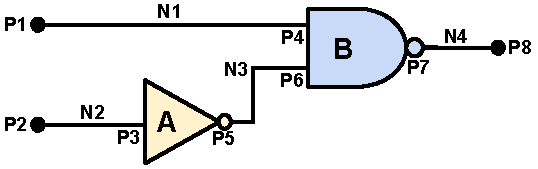
\includegraphics[width=0.7\linewidth]{img/tecnica/circuitExample}
%     % \caption{Combinational circuit portion with two logic gates (A and B), four nets (N1 to N4), and eight pins (P1 to P8).}
%     \caption[Fragmento de um circuito combinacional]{Fragmento de um circuito combinacional composto por duas portas lógicas (A e B), quatro nets (N1 a N4) e oito pinos (P1 a P8).}
%     \label{fig:circuito_exemplo}
% \end{figure}
%
% Um estimador de comprimento de interconexão deve ter acesso à informação de quais pinos pertencem a cada Net, bem como às posições dos pinos dentro do leiaute do circuito.
% A Figura~\ref{fig:classHierarchyOOD} ilustra uma possível decomposição para o problema de estimativa de comprimento de interconexão seguindo o modelo de programação \ac{ood}.
% Este diagrama é composto por dois módulos: \textit{Netlist} e \textit{Placemment}.
% O módulo \textit{Netlist} possui duas classes, \textit{Net} e \textit{Pin}, para descrever as interconexões do circuito e os pinos associados.
% Para a classe \textit{Pin}, este módulo caracteriza apenas o nome do pino e a rede a que ele pertence, sem qualquer informação de posicionamento.
% O módulo \textit{Placemment}, por sua vez, descreve as posições dos pinos.
% A seta entre as classes \textit{Pin} e \textit{Net} representam uma relação de agregação, o que significa que a interconeção possui uma referência aos seus pinos, enquanto um pino tem uma referência à sua interconeção proprietária.
% A seta entre as duas classes \textit{Pin} representa um relacionamento hierárquico, o que significa que a classe \textit{Pin} do módulo \textit{Placement} estende os atributos do pino do módulo \textit{Netlist}.
%
% \begin{figure}[ht]
%     \centering
%     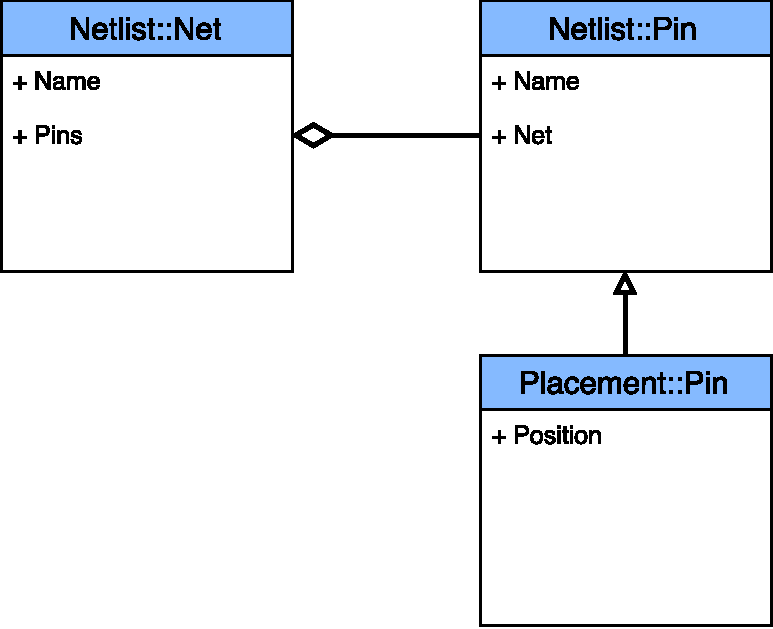
\includegraphics[width=0.5\linewidth]{img/tecnica/classHierarchyOOD}
%     % \caption{Class diagram to model wirelength estimation problem with \ac{ood} approach.}
%     \caption[Diagrama de classe com OOD]{Diagrama de classe para modelagem da estimativa do comprimento de uma intercenexão seguindo o modelo de programação \ac{ood}}
%     \label{fig:classHierarchyOOD}
% \end{figure}
%
% Embora possa ser fácil decompor um problema usando o modelo \ac{ood}, a implementação de um software, baseando-se apenas neste modelo de programação, pode levar a uma hierarquia de classes excessivamente complexa.
% Esta questão é particularmente crítica no desenvolvimento de uma biblioteca de software, pois é difícil prever, durante o design da biblioteca, como ela será realmente utilizada.
% Por exemplo, suponha que outro problema requer informações temporais sobre os pinos do circuito da Figura~\ref{fig:circuito_exemplo}.
% Seguindo o modelo de programação \ac{ood}, essas informações temporais podem ser adicionadas naturalmente criando um novo módulo chamado \textit{Timing} e uma nova classe \textit{Pin} (com atributos de temporização dos pinos) neste módulo.
% Por sua vez, esta nova classe deve também estender a classe \textit{Pin} do módulo \textit{Netlist}.
% Esta nova decomposição resulta na hierarquia de classes mostrada na Figura~\ref{fig:classHierarchyTimingOOD}.
%
% \begin{figure}[ht]
%     \centering
%     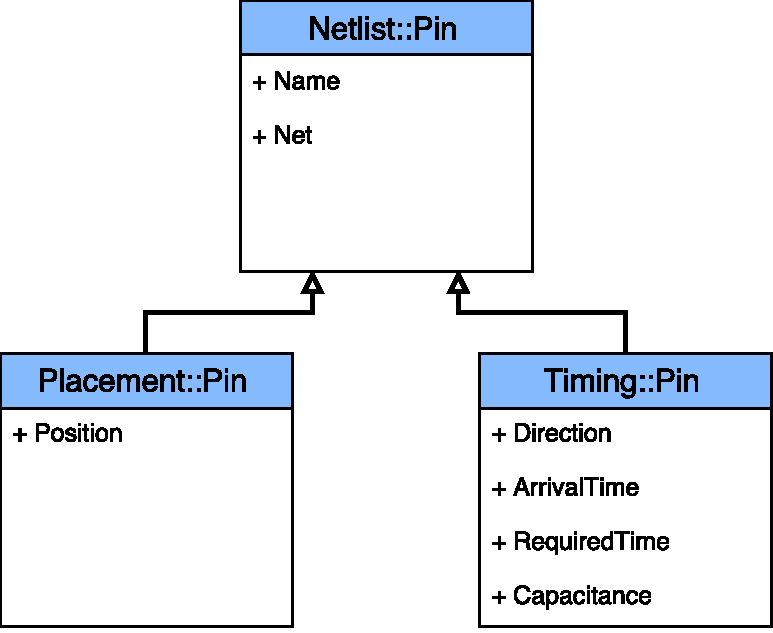
\includegraphics[width=0.5\linewidth]{img/tecnica/classHierarchyTimingOOD}
%     % \caption{Class diagram to model when pin timing information is added.}
%     \caption[Diagrama de classe de um pino]{Diagrama de classe de um pino com informações de posicionamento e temporais.}
%     \label{fig:classHierarchyTimingOOD}
% \end{figure}
%
%
% Agora, suponha que outro desenvolvedor queira usar nossa biblioteca de Physical Design para implementar um algoritmo de \ac{itdp}.
% Para fazer isso, este desenvolvedor irá precisar de uma nova classe \textit{Pin} com as informações de posicionamento e temporização.
% Em \ac{ood}, isso pode ser realizado através de herança múltipla, onde esta nova classe \textit{Pin} estende as classes \textit{Pin} de \textit{Placemment} e \textit{Timing}.
% No entanto, a herança múltipla não é suportada por todas as linguagens de programação, e mesmo quando suportada, não é recomendável porque pode levar a problemas de design~\cite{nystrom2014game}.
%
% Sem recorrer a herança múltipla, a solução consiste em criar uma nova classe \textit{Pin} que se estende do módulo \textit{Placement} ou \textit{Timing}, e repita o código da outra classe (que não foi estendida).
% Esta solução está apresentada na Figura~\ref{fig:classITDP}(a) e~\ref{fig:classITDP}(b).
% De qualquer forma, não existe uma maneira simples de reutilizar informações de posicionamento e tempo sem ocorrer replicação de código.
% A única opção restante é reunir todas as informações na classe \textit{Pin} do módulo \textit{Timing}, fazendo o mesmo estender o do módulo \textit{Placement}.
% Esta solução está ilustrada na Figura~\ref{fig:classITDP}(c).
% No entanto, nem sempre é necessário ter informações de posicionamento no módulo \textit{Timing}.
% Por exemplo, uma ferramenta analize de timing estática pode não precisar de informações de posicionamento durante etapas iniciais do projeto.
% Portanto, a adoção da última solução (Figura~\ref{fig:classITDP}(c)) levaria ao desperdício de memória, uma vez que informações desnecessárias seriam armazenadas.
%
% \begin{figure}[!ht]
%     \centering
%     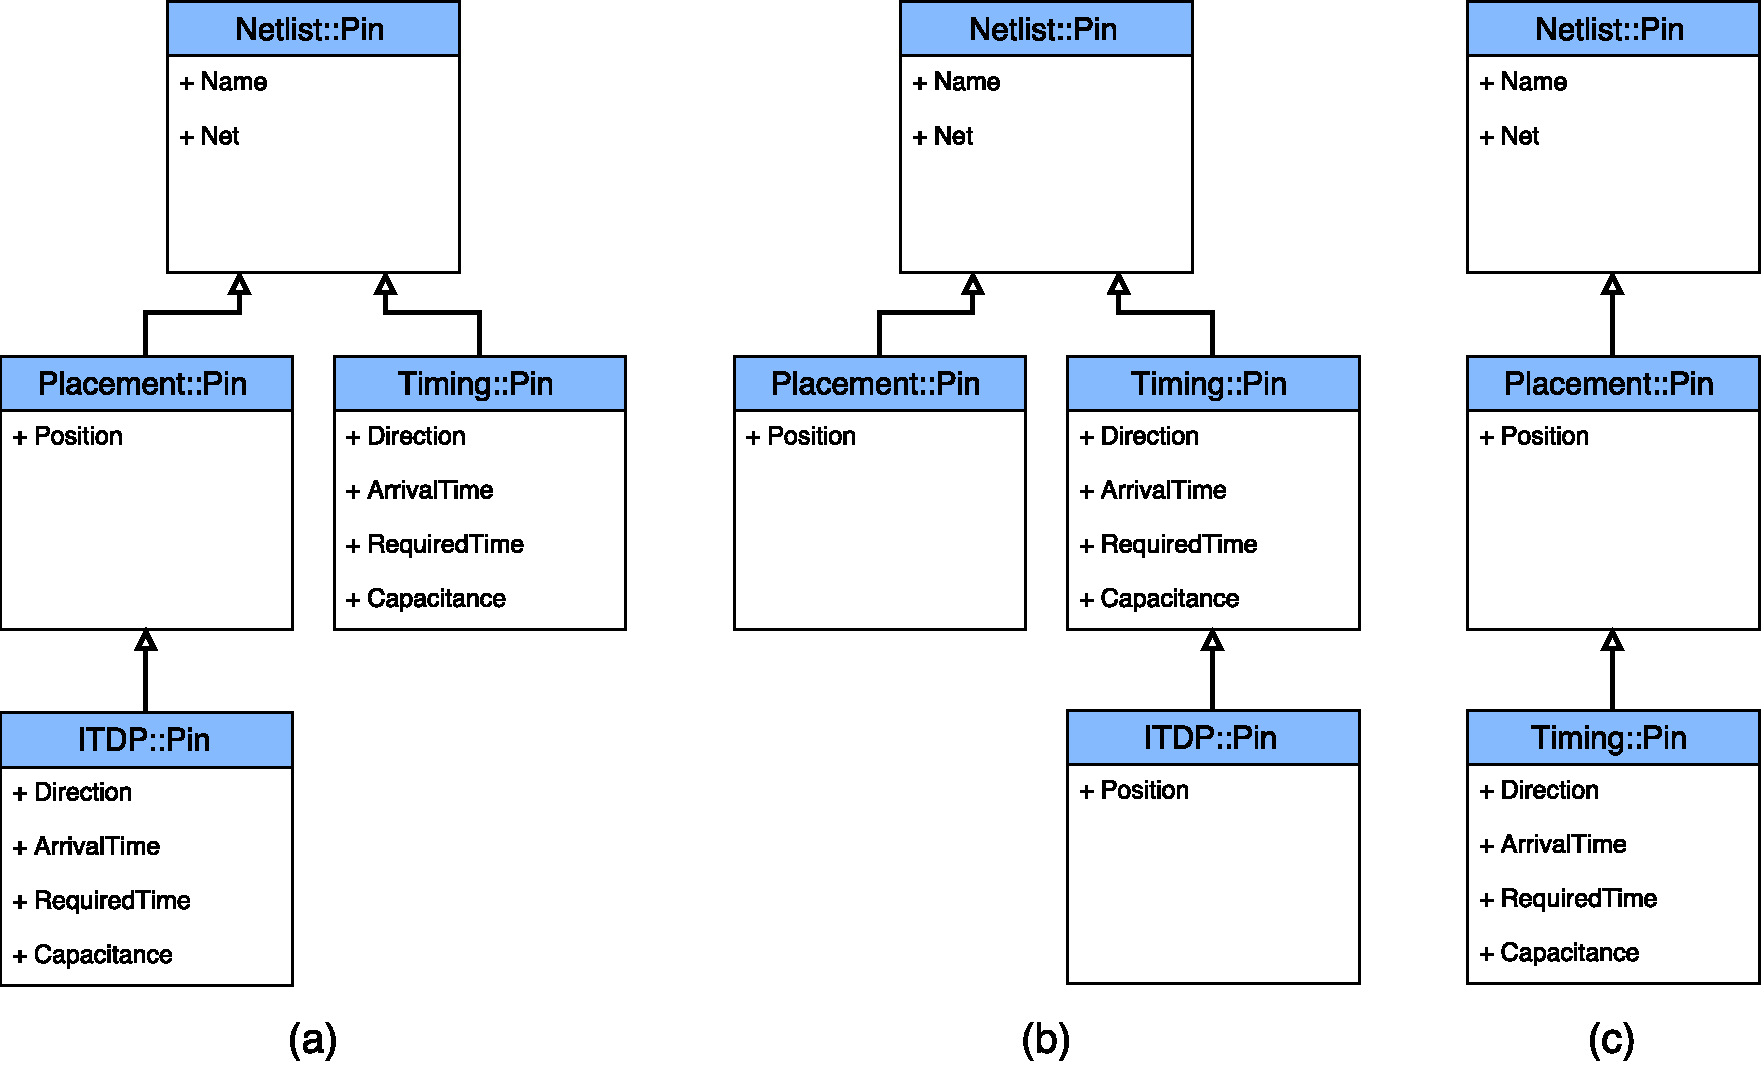
\includegraphics[width=\textwidth]{img/tecnica/ITDPsolutionOOD}
%     % \caption{Possible class hierarchy to support information of \textit{Timing} and \textit{Placement} for a timing-driven placement algorithm following \ac{ood} approach.}
%     \caption[Hierarquia de classes para suportar \textit{Timing} e \textit{Placement}]{Possível hierarquia de classes para suporte  informações de \textit{Timing} e \textit{Placement} para um algorítmo de \ac{itdp} seguindo o modelo de programação \ac{ood}.}
%     \label{fig:classITDP}
% \end{figure}




% \section{Modelo de Programação Orientado a Dados}
% \label{sec:modelo_orientado_dados}
%
% \section{Modelagem dos Dados para Physical Design}
% \label{sec:modelagem_physical_design}

% \subsection{Estudo de Caso A\@: Verificação dos Limites do Chip}
% \label{subsec:problema_A}

% \subsection{Estudo de Caso B\@: Estimativa de Interconexão}
% \label{subsec:problema_B}

% \subsection{Estudo de Caso C\@: Clusterização de Registradores}
% \label{subsec:problema_C}


% apresentar modelo de memoria
% apresentar como cache miss funciona
% apresentar ood
% apresentar limitação do ood
% apresentar dod
% apresentar entity system
% Discutir como o DOD reduz o numero de cache misses
% como aplicar o dod em problemas
%     Problema A - limites do chip
%         como seria modelado OOD
%         como seria modelado DOD
%     Problema B - interconexão
%         como seria modelado OOD
%         como seria modelado DOD
%     Problema C - cluster
%         como seria modelado OOD
%         como seria modelado DOD
